\documentclass[12pt]{article}
\usepackage{amsmath}
\usepackage{setspace}
\usepackage{adjustbox}
\usepackage{graphicx}
\usepackage{float}
\usepackage{multicol}
\usepackage{hyperref}
\usepackage{subfig}
\usepackage{wrapfig}
\usepackage{xcolor}
\usepackage{tabularray}
\usepackage{sidecap}
%\usepackage{natbib,url}
\usepackage[backend=biber,style=numeric,maxnames =2,giveninits = true]{biblatex}
\addbibresource{journal_abbreviations.bib}
\addbibresource{References.bib}
\usepackage[margin = 1in]{geometry}
\usepackage{fancyhdr}
\usepackage{sectsty}
\usepackage{titlesec}


\sectionfont{\fontsize{14}{15}\selectfont}
\subsectionfont{\fontsize{12}{15}\selectfont}
%\bibliographystyle{abbrv}
\DeclareBibliographyDriver{std}{%
  \usebibmacro{bibindex}%
  \usebibmacro{begentry}%
  \usebibmacro{author/editor+others/translator+others}%
  \usebibmacro{title}%
  \setunit{\labelnamepunct}\newblock
  %\usebibmacro{title}%
    %\newunit\newblock
  \usebibmacro{journal}
  \newunit\newblock
  \usebibmacro{date}%
  \newunit\newblock
\usebibmacro{finentry}}

\DeclareBibliographyDriver{stdbook}{%
  \usebibmacro{bibindex}%
  \usebibmacro{begentry}%
  \usebibmacro{author/editor+others/translator+others}%
  \setunit{\labelnamepunct}\newblock
  %\usebibmacro{title}%
  \usebibmacro{title}
  \newunit\newblock
  \usebibmacro{date}%
  \newunit\newblock
\usebibmacro{finentry}}

%\DeclareBibliographyAlias{article}{std}
%\DeclareBibliographyAlias{book}{stdbook}
%\DeclareBibliographyAlias{misc}{stdbook}
\AtEveryBibitem{% Clean up the bibtex rather than editing it
 \clearfield{isbn}
 \clearfield{doi}
 \clearfield{url}
 \clearfield{issn}
 }
\AtBeginBibliography{\small}
\definecolor{gray_c}{rgb}{0.745, 0.898, 0.898}
\definecolor{gray_h}{rgb}{0.43, 0.72, 0.72}

%\titlespacing\section{0pt}{12pt plus 4pt minus 2pt}{0pt plus 2pt minus 2pt}
\titlespacing\subsection{0pt}{12pt plus 4pt minus 2pt}{0pt plus 2pt minus 2pt}
%\titlespacing\subsubsection{0pt}{12pt plus 4pt minus 2pt}{0pt plus 2pt minus 2pt}

\def\epo{\epsilon\rightarrow 0}
\def\lb{\left(}
\def\rb{\right)}
\def\ls{\left[ \vphantom]}
\def\rs{\right] }
\def\ep{\epsilon}

\title{Direct simulation of ocean-ice coupling in icy moons}
\author{Tobias Oliver}
\date{}

\begin{document}
\pagestyle{fancy}
\thispagestyle{fancy}
%... then configure it.
\fancyhf{} % clear all header fields
\fancyhead[L]{\textcolor{red}{Tobias Oliver\\
Research Proposal}}
\fancyfoot[R]{\thepage}
\newcommand{\citep}[1]{\cite{#1}}
\begin{center}
\large{\textbf{Ocean-ice coupling on icy moons}}
\end{center}
%\maketitle
%\section{Summary}
%I propose to study two processes important to the interaction between the ocean and ice on the ``ocean worlds'' of the Jovian and Saturnian system. Forward, numerical simulations will be used to better constrain the dynamics of the sub-surface oceans on these planets. A focus is placed on two models that will couple ocean dynamics to the ice, so that surface observations from the upcoming \textit{Europa Clipper} and \textit{JUICE} missions can be used to predict ocean dynamics.
%First, I will study a conjugate heat transfer model in which the surface response to underlying convection is directly simulated. No prior simulations of this type exist in the planetary literature. Second, I will investigate a double diffusive model, involving the coupled dynamics of solutal and thermal buoyancy. This process is thought to be particularly important near the ocean-ice interface where melting ice releases cold, fresh water into the underlying ocean.

I propose to study the effects of salinity on convective processes in the icy moons of Jupiter and Saturn. 
I will investigate the interplay of horizontal and bottom driven convection, and the competing effects of temperature and salinity via a suite of tailored numerical simulations. 
A focus will be placed on the interaction between the subsurface oceans and the overlaying ice, so that predictions can be made about surface processes. 
\textbf{With upcoming data from the \textit{Europa Clipper} and \textit{JUICE} missions, the results from this study can be used to relate surface observations to ocean dynamics}.

\section{Background}
The solar system contains a number of icy bodies, many of which are thought to be ``ocean worlds,'' that may be suitable candidates for the habitability of life.
Europa, Callisto, and Ganymede, as well as the Saturnian moons Enceladus and Triton, were all identified as likely ocean worlds after data began to return from the \textit{Galileo} and \textit{Cassini} missions \citep{fN16}.
The sub-surface oceans link the solid cores of these moons to their icy exteriors, and are therefore expected to play an important role in the transport of heat and chemicals to their surfaces \citep{kS20}. 
Figure \ref{f:pic}(a) illustrates a proposed structure.

%Both gravity and magnetic measurements aided in the discovery, but in the case of Europa, the latter proves more convincing. 
%Since the magnetic dipole of Jupiter is tilted about $10^{\circ}$ with respect to the orbital plane, the Jovian moons experience a magnetic induction as they orbit the planet.
%Induced magnetic fields were measured by \textit{Galileo}, and it has been determined that a conducting ocean near the surface is likely necessary to explain observations\citep{fN16,cZ00}. 

It is likely that the oceans are turbulent and capable of convecting a large amount of heat and chemicals between the solid interior and icy crust.
%A variety of forcing mechanisms have been proposed and discussed, such as electromagnetic coupling\citep{cGlP19}, tides, and precession\citep{kS24}, and in this investigation 
I propose to study buoyantly driven flows, in which variations in the fluid density drive convection.
Density variations are usually attributed to two separate mechanisms-- heterogeneities in temperature and salinity. The associate density variations drives convection and references \citep{yA21,wK22} predict that this mechanism serves to flatten the ice shell of Europa (ie.  homogenous thickness).
%\begin{wrapfigure}{R}{0.6\textwidth}
%\end{wrapfigure}
\begin{figure}[H]
	\begin{center}
		\subfloat[][]{\includegraphics[width=0.25\textwidth]{figures/europa_ice}}
		\quad
		\subfloat[][]{\includegraphics[width=0.35\textwidth]{figures/hc}}
	\subfloat[][]{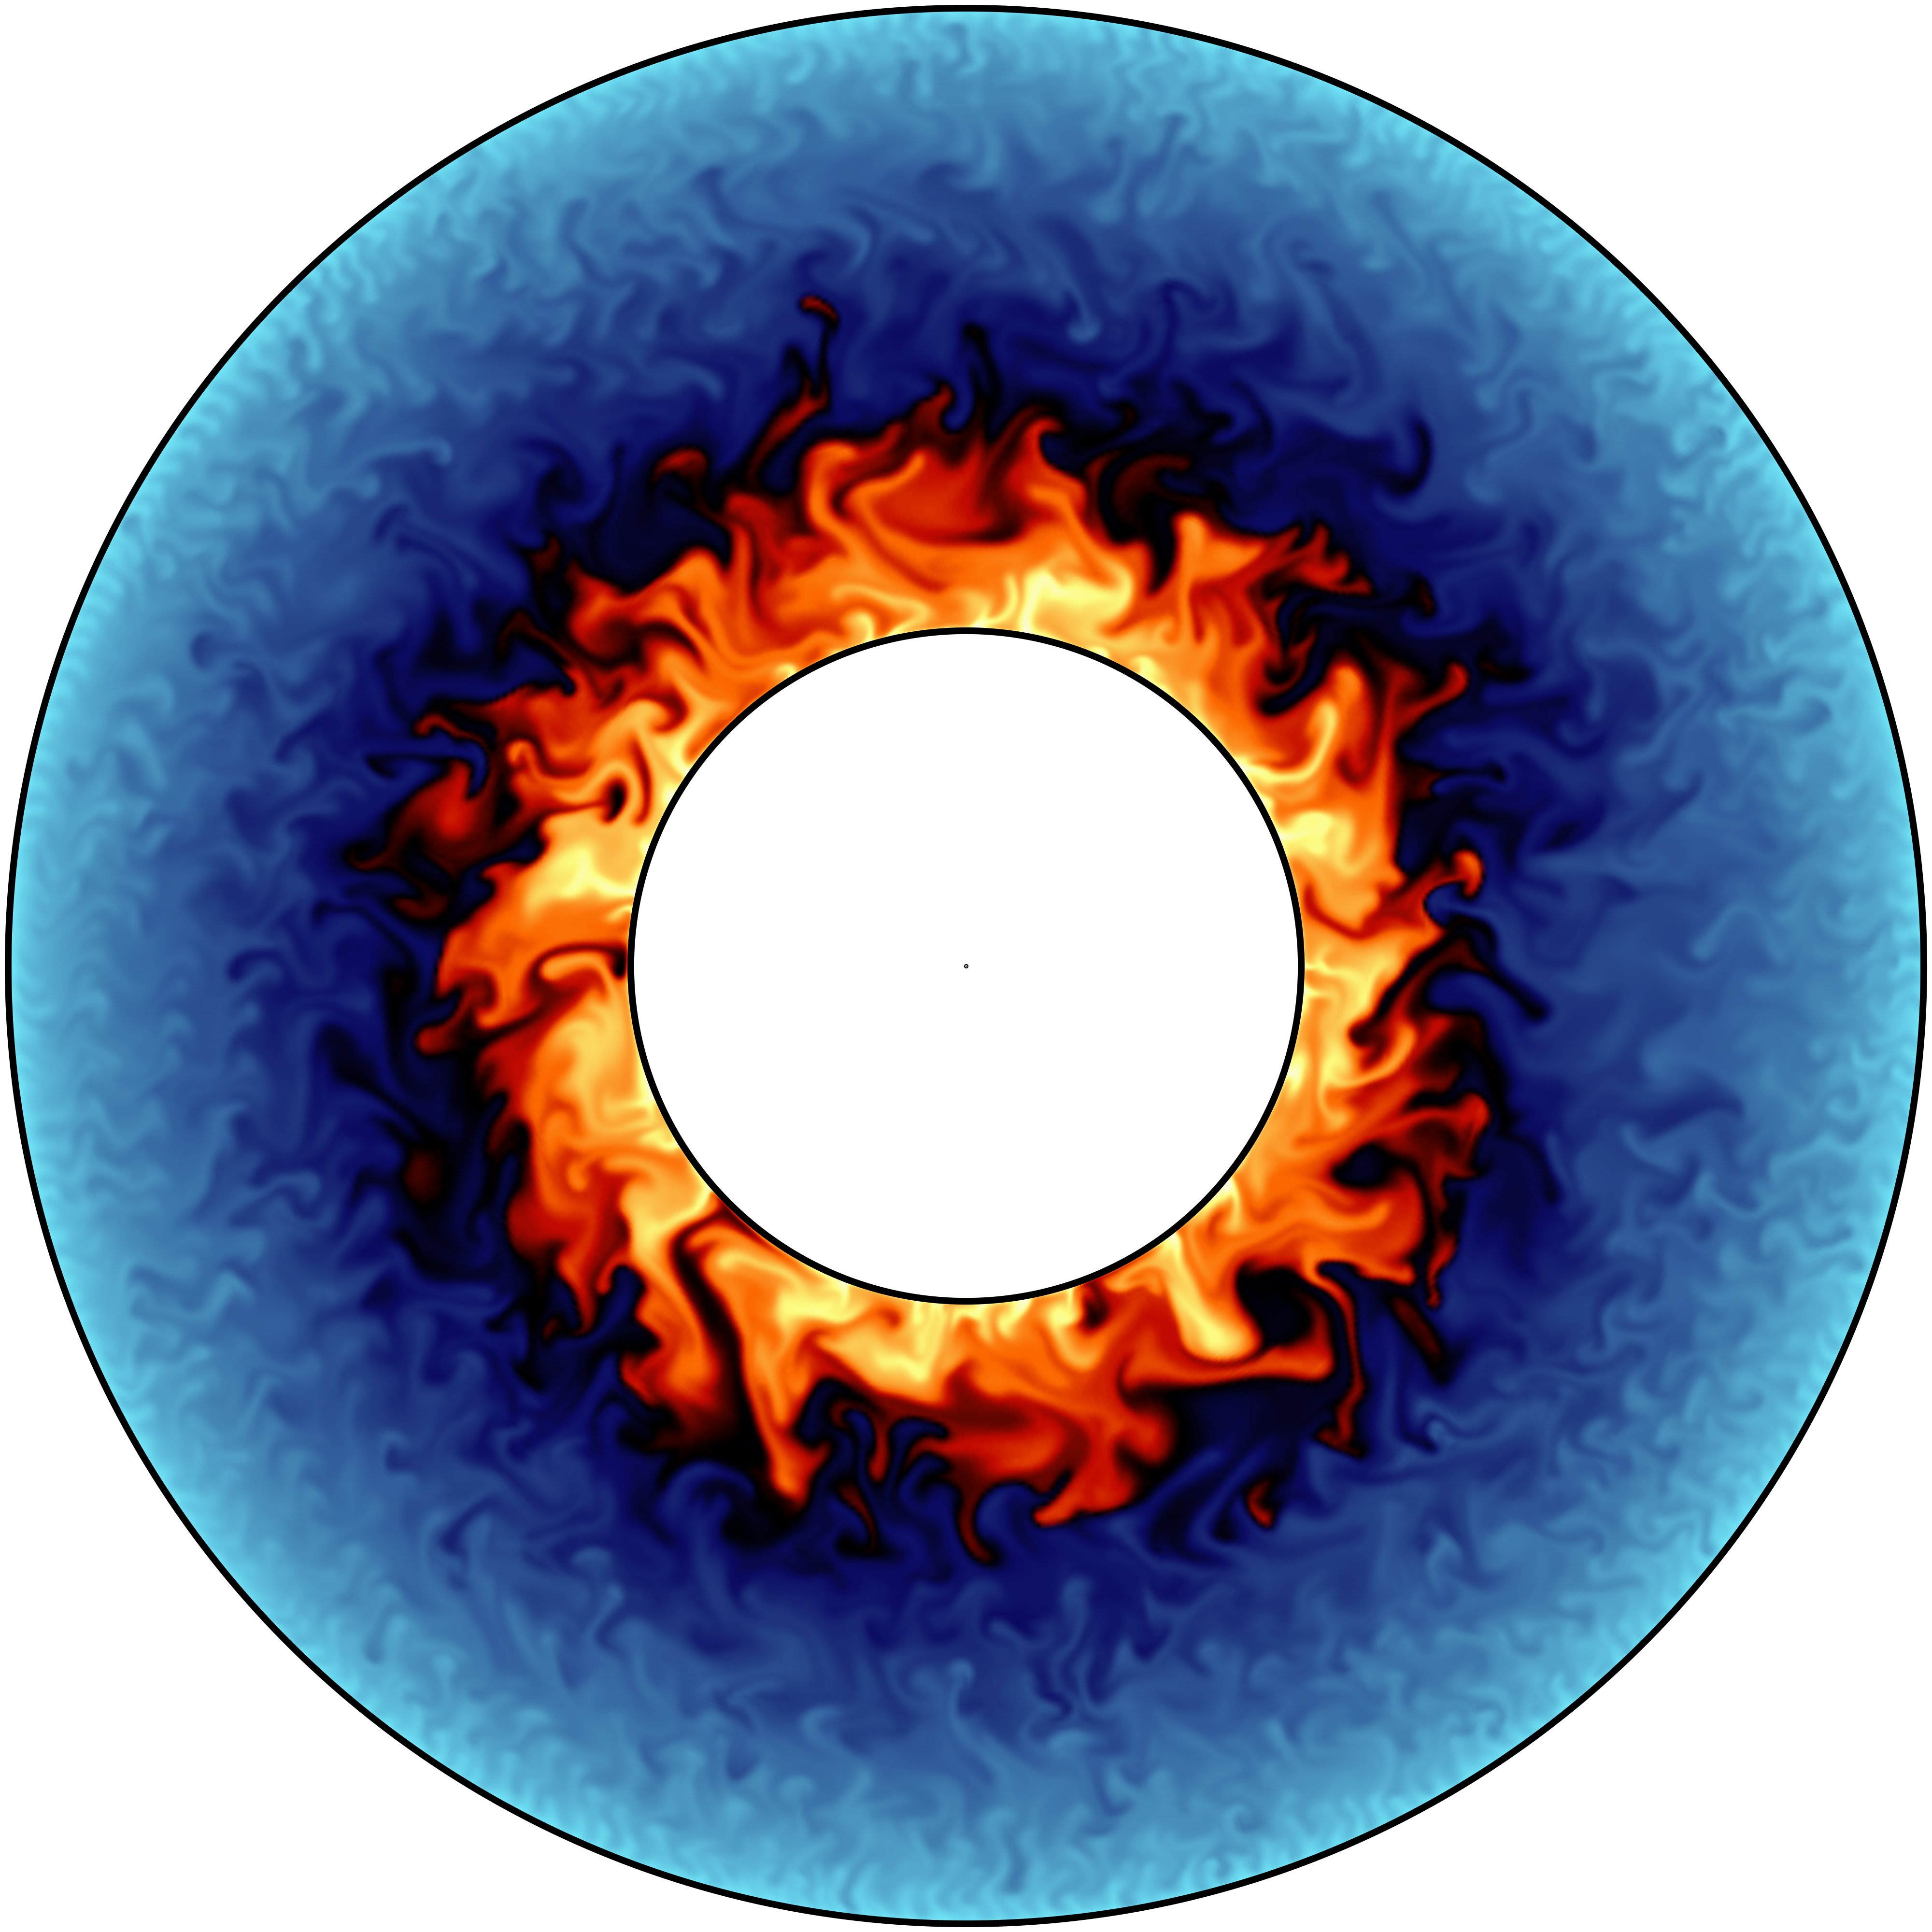
\includegraphics[width=0.25\textwidth]{figures/conv}}
	\end{center}
	\caption{(a) Artist interpretation of subsurface ocean on Europa, not to scale (NASA/JPL-Caltech). (b) Possible mechanism for horizontal convection driven by heterogenous melting. Adapted from \citep{wK22}. Simulation (by author) of thermal bottom driven convection in a planetary core\citep{tO25}.}
	\label{f:pic}
\end{figure}

Two different mechanisms for convection will be considered.
Horizontal convection (HC) results from density heterogeneities about the icy surface (see figure \ref{f:pic}(b)). Heavy fluid sinks and light fluid flows in to replace it. This drives a circulations within the ocean. Bottom driven convection (BDC) is due to density differences between the silicate core and the icy surface. Lighter fluid near the core rises while heavier surface fluid sinks, once again setting up a circulation. In plane layers, BDC is often referred to as Rayleigh-B\'enard convection. On icy moons latitudinal variations in melt are expected to drive HC \citep{wK22}, whereas radiogenic heating from the silicate core \citep{kS14,kS19,jK22} likely drives BDC. A snapshot of a simulation of BDC in a planetary interior is shown in figure \ref{f:pic}(c)\citep{tO25}. The competition between these two mechanisms has receieved little attention because it is difficult to simultaneously model both processes in a consistent manner.


\section{Proposed project and methodology}

\textbf{In this project I propose to study the interaction of the icy shell with the convecting ocean via numerical simulations of a coupled ice-ocean system.} 
Primarily, I will focus on the heat flux through the icy shell, and use these results to make predictions about about total flux in the icy moons, as well as the latitudinal dependence. These predictions will be verifiable by the \textit{Europa Clipper} and \textit{JUICE} missions.

There are two major challenges associated with this study. The first is that it is not possible to perform fluid simulations in the actual parameter regimes of the icy moons. The second is generating a consistent model for heat fluxes into the ice and the resulting melt and release of fresh water.
\subsection{Convection parameters of the icy moons}
In convection studies, we attempt to solve the dynamical equations governing conservation of energy, momentum, and salinty. However, there is a large disparity between the scales relevant to planetary bodies and the scales that can be realistically simulated. 
Usually this issue is formalized in terms of non-dimensional numbers that reflect ratios of the magnitudes of forcing mechanisms. %Alterntively, we can think of these quantities as ratios of different forcing terms in the governing equations. 
%In a geophysical and astrophysical context, there are two non-dimensional numbers of particular importance: the Rayleigh and Ekman numbers. 
The Rayleigh number $Ra$ describes the ratio of buoyancy to diffusivity. For planetary bodies, $Ra$ is very large, generally indicating vigourous convection.
The Ekman number $Ek$ approximates the ratio of viscous diffusion to Coriolis effects. Values for $Ek$ tend to be very small, indicating that rotation plays an important role.
For salty oceans, a buoyancy ratio $\Gamma$ is necessary to prescribe the relative effects of temperature and buoyancy on density.
%Two other quantities of importance are the Nusselt number, $Nu$, and Prandtl number, $Pr$. 
%They are the ratio of total heat transfer to conductive heat transfer and the ratio of momentum to thermal diffusivity respectively \citep{kS19}. 
Explicitly, these parameters are
\[Ra = \frac{g\alpha\Delta T D^{3}}{\nu\kappa_{T}}\quad Ek = \frac{\nu}{\Omega D^{2}}\quad \Gamma = \frac{\alpha\Delta T}{\beta \Delta S}\]% \quad Nu = \frac{hD}{k_{O}} \quad Pr= \frac{\nu}{\kappa_{T}},\]
where $g$ is the surface gravitational acceleration, $\alpha$ and $\beta$ are the coefficient of thermal and solutal expansion respectively, $D$ is the ocean thickness, $\nu$ and $\kappa_T$ are the diffusivities of momentum and temperature respectively, and $\Omega$ is the planetary rotation rate.
%, $h$ is the total heat transfer, and $k_O$ is the thermal conductivity of the ocean. 
$\Delta T$ is the temperature difference between the ocean surface and floor. $\Delta S$ is the average ocean salinity. 

%A compositional Rayleigh number $Ra_{S}$ can be defined by replacing $\alpha, \Delta T,\text{ and, }\kappa_{T}$ with the associated quantities for salinity.

To take Europa as an example, predicted values of $Ra$ and  $Ek$ are $O\lb 10^{20}\rb $ and $O\lb 10^{-12}\rb $ respectively. $\Gamma$ is poorly constrained but is much less than unity \citep{yA21}. In the context of icy moons, numerical simulations have only reached values of $Ra \sim 10^{8}$ and $Ek \sim 10^{-5}$\citep{dL23}. 
%In studies of different planetary bodies, more aggressive simulations have been performed (eg. figure \ref{f:pic}(b), references \citep{tO25}), however all fall significantly short of reaching realistic values. For icy moons, it is particularly difficult to reach small values of $Ek$ because the ocean depth is much smaller than the planetary radius. 
The procedure, therefore, is to attempt to establish scaling laws with the non-dimensional parameters by simulating at moderate values, and then extrapolating to planetary values.

I will explore similar parameters to the regimes studied in references \citep{dL23,kS19}. This will allow me to best compare these ``purely thermal'' results to my findings, which will better elucidate the new effects of saline convection. $\Gamma$ will be swept across two orders of magnitude in order to establish a scaling relationship with the buoyancy ratio. A complete list of the proposed simulations is given in table \ref{t:param}. 
\subsection{Coupling the ice and ocean}

Horizontal convection is likey driven by salinity variations about the outer boundary of the liquid domain. In order to investgate this mechanism, it is necessary to couple the heat fluxes into the ice with melt into the ocean. 
Convective studies that do not consider salinity have generally only investigated the ocean domain\citep{kS19,dL23}. The general approach is to fix the temperature of the bounding surface (ice shell), however this implies uniform melt.
\textbf{I propose to use a simulation configuration in which the ice is included in the solution domain so that heat is able to conduct from the ocean into the ice.}
A boundary condition for temperature is placed on the moon surface, and the temperature of the ocean-ice interface is allowed to vary. The interfacial temperature can be used to determine the salinity\citep{wK22}.

The addition of the ice layer introduces a fourth non-dimensional parameter to consider. The Biot number, $Bi$\citep{jL24} represents the ratio of conductive resistance to convective heat flow and governs the ice-ocean temperature response. 
In our simulations $Bi$ is an output value, but we can control it by varying $D_{i}$, the thickness of the ice layer. Estimates for Europa suggest $Bi \sim O\lb 10^{6}\rb$\citep{dL23} which is not numerically feasible. Therefore, I propose to simulate at two different values of $D_{i}$ to determine scaling behavior with $Bi$ to extrapolate to the icy moons. 

%Most convective studies have investigated only the ocean domain\citep{kS19, dL23}. The fixed melting temperature of ice is prescribed at the fluid domain boundary.
%%and have prescribed boundary conditions at the ocean-ice interface to represent the fixed melting temperature of the ice. 
%A forward model with a melting icy boundary was used to constraing ice topography, but the fast timescale heat fluctuations in the icy shell were not investigated\citep{jK24}.

%A model with a dynamic, melting icy boundary has been studied, however the authors were primarily interested in the resulting topography. The fast timescale heat fluctuations in the icy shell due to the underlying convection were not investigated\citep{jK24}. 

%CHT is a simulation configuration in which a solid boundary is included in the solution domain so that heat is able to conduct from the fluid into the boundary. Rather than placing a boundary condition on the fluid surface, the condition is placed on the outermost solid surface and the liquid and solid domains are solved together\citep{dA09}. Whether CHT is important can be estimated by the value of the Biot number $Bi$ \citep{dA09,jL24}, a non-dimensional parameter representing the ratio of conductive resistance to convective heat flow. For the conjugate problem, $Bi$ can be estimated as
%\[Bi \sim Nu\frac{k_{f}}{k_{i}}\frac{D_{i}}{D},\]
%where $k_{f\lb i\rb }$ is the thermal conductivity of the fluid (ice) and $D_{i}$ is the ice depth.
%Estimates for Europa therefore suggest $Bi \sim O\lb 10^{6}\rb$\citep{dL23}. When $Bi>1,$ the conjugate problem is considered relevant, and therefore this process likely plays a role in the evolution of icy shells.

\begin{table}
\begin{center}
\begin{tabular}{|c|c|c|c|c|c|}
\hline
$Ra$&$Ek$&$D_{i}/D$& $\Gamma$ &\# Simulations & Cost (cpu$\times$hour)\\
		\hline
$\lb 5 \times 10^{6} - 2 \times 10^{8} \rb $ & $3 \times 10^{-4} $ & $0.5,0.1$&0.5,0.05&20&$1.7 \times 10^{6}$\\
  	\hline
$\lb 5 \times 10^{6} - 1 \times 10^{9} \rb $ & $1 \times 10^{-4} $ & $0.5,0.1$&0.5,0.05&20&$1.7\times 10^{6}$\\
  	\hline
$\lb 5\times 10^{7}, 2 \times 10^{9} \rb $ & $3 \times 10^{-5} $ & $0.5,0.1$&0.5,0.05&8&$2.5\times 10^6$\\
		\hline
%Shell & $10^5$& $\infty$&$10^4-10^5$& 5& $2\times 10^{6}$\\
%		\hline
%Shell & $10^5$& $10^{-4}$&$10^4-10^5$& 5& $2\times 10^{6}$\\
%		\hline
%Plane &$5\times10^{5}-2\times10^{6}$ & $3\times10^{-4}$&$12.5Ra$ &5 &$2.5\times 10^{5}$  \\
%		\hline
%Plane &$10^{6}-10^{7}$ & $10^{-4}$&$12.5Ra$& 5 & $5\times 10^{5}$\\
%		\hline
%Plane &$10^{7}-5\times 10^{7}$ & $3\times10^{-5}$&$12.5Ra$ & 5& $10^{6}$ \\
		\hline
Totals & & & &48&$4.9 \times 10^6$ \\
		\hline
\end{tabular}
\end{center}
\caption{Proposed parameter space. The third column presents the ratio of ice to ocean thickness, which can be modified to change $Bi$. Computing costs are estimate values based off of existing studies \citep{dL23,rM19} and personal experience with relevant codes.}
\label{t:param}
\end{table}

%\begin{table}
%\begin{center}
%\begin{tabular}{|c|c|c|c|c|c|}
%\hline
%Geometry&$Ra$&$Ek$&$D/D_{i}$ or $Ra_S$ &\# Simulations & Cost (cpu$\times$hour)\\
%		\hline
%Shell&$\lb 5 \times 10^{6} - 2 \times 10^{8} \rb $ & $3 \times 10^{-4} $ & $2,10$&10&$7 \times 10^{5}$\\
%		\hline
%Shell&$\lb 5 \times 10^{6} - 1 \times 10^{9} \rb $ & $1 \times 10^{-4} $ & $2,10$&10&$1\times 10^{6}$\\
%		\hline
%Shell&$\lb 5 \times 10^{7} - 2 \times 10^{9} \rb $ & $3 \times 10^{-5} $ & $2,10$&10&$2\times 10^6$\\
%		\hline
%Shell & $10^5$& $\infty$&$10^4-10^5$& 5& $2\times 10^{6}$\\
%		\hline
%Shell & $10^5$& $10^{-4}$&$10^4-10^5$& 5& $2\times 10^{6}$\\
%		\hline
%Plane &$5\times10^{5}-2\times10^{6}$ & $3\times10^{-4}$&$12.5Ra$ &5 &$2.5\times 10^{5}$  \\
%		\hline
%Plane &$10^{6}-10^{7}$ & $10^{-4}$&$12.5Ra$& 5 & $5\times 10^{5}$\\
%		\hline
%Plane &$10^{7}-5\times 10^{7}$ & $3\times10^{-5}$&$12.5Ra$ & 5& $10^{6}$ \\
%		\hline
%Totals & & & & 55&$9.5 \times 10^6$ \\
%		\hline
%\end{tabular}
%\end{center}
%\caption{Proposed parameter space. The fifth column presents the ratio of ocean to ice thicknesses for the CHT model and the compositional Rayleigh number for the DDC model. 
%Computing costs are estimate values based off of existing studies \citep{rM19,rM17,dL23,jF24} and personal experience with relevant codes.}
%\label{t:param}
%\end{table}
\subsection{Proposed simulations and computing requirements}
I propose a suite of 48 simulations to investigate ice-ocean coupling in the icy moons. The specific parameter values are given in table \ref{t:param}, as well as the estimated computing cost. Computing time is based on previous rotating convection studies in icy moons \citep{dL23}, but because the proposed simulation framework is novel, these values should be considered as rough estimates. The existing hydrodynamics code \texttt{Nek5000}\citep{nek5000} will be used to perform the simulations, and can be congifured to handle thermal-saline convection as well as the solid icy domain.
All simultions will be performed in spherical shells to best represent the icy moon geometry.
 I will apply for computing time through ACCESS and TACC, which are both supported by the National Science Foundation. I will also apply for local computing resources depending on the host institution.
 \subsection{Timeline}
 Significant effort will be required to build and test the numerical model, which I expect to take a year. This will include building and testing a simplified planar model which can be used to gauge the feasability of the proposed parameter regime. Planar models are generally much cheaper to simulate. If the proposed parameters are determined to be too extreme for the available computing time, then the most expensive simulations (low $Ek$) will be relegated to the cheaper planar model. Codes and methods to analyze the output will be developed during this time. The second year will be dedicated to performing the simulations in table \ref{t:param} and investigating the differences between pure BDC and coupled BDC and HC. In the third year, I will focus on developing predicitions that can be made by \textit{Europa Clipper} and \textit{JUICE} based on my results.%\begin{figure}

%	\begin{center}
%		\includegraphics[width=0.7\textwidth]{figures/reg_diagram}
%		\phantom{Lorem ipsum dolor sit amet}
%	\end{center}
%	\caption{Regime diagram for rotating convection, adapted from \citep{dL23,tG16}. The region left of the solid black line represent simulation results for a Europa-like geometry\citep{aB22}. The region right of the black line represents scaling predictions from \citep{tG16}. Dashed lines - extrapolations of asymptotic predictions into the DNS region. Crosses and stars - parameter space from Lemasquerier et al. 2023\citep{dL23} and Soderlund 2019\citep{kS19} respectively. Regions enclosed by dotted lines represent approximate parameter space for Europa and Ganymede \citep{dL23,kS19}. Red markers indicate proposed simulations for conjugate heat transfer (CHT) study.
%	}
%	\label{f:reg_d}
%\end{figure}


%There is a large disparity between the scales relevant to planetary bodies and the scales that can be realistically simulated.
%%In simulating geophysical flows, there is often a large disparity between the spatial and temporal scales relevant to planetary bodies, and the scales that we can realistically compute. 
%Usually this issue is formalized in terms of non-dimensional numbers that reflect ratios of the magnitudes of forcing mechanisms. %Alterntively, we can think of these quantities as ratios of different forcing terms in the governing equations. 
%%In a geophysical and astrophysical context, there are two non-dimensional numbers of particular importance: the Rayleigh and Ekman numbers. 
%The Rayleigh number $Ra$ describes the ratio of buoyancy to diffusivity. For planetary bodies, $Ra$ is very large, generally indicating vigourous convection.
%The Ekman number $Ek$ approximates the ratio of viscous diffusion to Coriolis effects. Values for $Ek$ tend to be very small, indicating that rotation plays a dominant role.
%Two other quantities of importance are the Nusselt number, $Nu$, and Prandtl number, $Pr$. 
%They are the ratio of total heat transfer to conductive heat transfer and the ratio of momentum to thermal diffusivity respectively \citep{kS19}. 
%Explicitly, these parameters are
%\[Ra = \frac{g\alpha\Delta T D^{3}}{\nu\kappa_{T}}\quad Ek = \frac{\nu}{\Omega D^{2}} \quad Nu = \frac{hD}{k_{O}} \quad Pr= \frac{\nu}{\kappa_{T}},\]
%where $g$ is the surface gravitational acceleration, $\alpha$ is the coefficient of thermal expansion, $D$ is the ocean thickness, $\nu$ and $\kappa_T$ are the diffusivities of momentum and temperature respectively, $\Omega$ is the planetary rotation rate, $h$ is the total heat transfer, and $k_O$ is the thermal conductivity of the ocean. $\Delta T$ indicates the temperature between the ocean surface and floor. 
%A compositional Rayleigh number $Ra_{S}$ can be defined by replacing $\alpha, \Delta T,\text{ and, }\kappa_{T}$ with the associated quantities for salinity.
%%Definitions and approximate values of these parameters are given in table \ref{t:nondim}.
%%\begin{table}
%%\begin{center}
%%\begin{tabular}{|c|c|c|c|c|c|c|}
%%\hline
%%Values&$Ra$ &$Ek$ &$Nu$ & $Pr$ &$Bi$ &$Le$\\
%%\hline
%%Definition&$\frac{g\alpha\Delta T D^{3}}{\nu\kappa_{T}}$& $\frac{\nu}{D^{2}\Omega}$ %Ra,Ek
%%	  &$\frac{hD}{k_o}$ &$\frac{\nu}{\kappa_{T}}$ %Nu,Pr
%%	  &$\frac{hD_i}{k_{i}}$ &$\frac{\kappa_{T}}{\kappa_{S}}$\\%Bi,Le
%%	  \hline
%%\end{tabular}
%%\end{center}
%%\caption{Definitions of non-dimensional parameters. $g$ is the surface gravitational acceleration, $\alpha$ is the coefficient of thermal expansion, $D$ is the ocean thickness, $\nu$ and $\kappa$ are the diffusivities of momentum and temperature respectively, $\Omega$ is the planetary rotation rate, $h$ is the total heat transfer, and $k_o(i)$ is the thermal conductivity of the ocean (ice). $\Delta T$ indicates the temperature between the ocean surface and floor. Approximate values for icy moons shown in figure \ref{f:reg_d}}.
%%\label{t:nondim}
%%\end{table}
%%\begin{SCtable}[50]%{l}{5.5cm}
%%	%\begin{adjustbox}{minipage=\linewidth,bgcolor={gray_c}}
%%%\begin{tabular}{|c|c|}
%%	\large
%%\begin{tblr}{
%%    colspec = {|c|c|},
%%    row{1} = {gray_h},
%%    row{2-7} = {gray_c},
%%  }
%%\hline
%%Parameter&Definition\\%$Ra$ &$Ek$ &$Nu$ & $Pr$ &$Bi$ &$Le$\\
%%\hline
%%$Ra$&$\frac{g\alpha\Delta T D^{3}}{\nu\kappa_{T}}$\\
%%\hline
%%$Ek$ &$\frac{\nu}{D^{2}\Omega}$\\
%%\hline
%%$Nu$&$\frac{hD}{k_O}$\\
%%\hline
%%$Pr$&$\frac{\nu}{\kappa_{T}}$\\
%%\hline
%%$Bi$ &$\frac{hD_i}{k_{i}}$\\
%%\hline
%%$Le$ &$\frac{\kappa_{T}}{\kappa_{S}}$\\
%%\hline
%%%\end{tabular}
%%\end{tblr}
%%\caption{Definitions of non-dimensional parameters. $g$ is the surface gravitational acceleration, $\alpha$ is the coefficient of thermal expansion, $D$ is the ocean thickness, $\nu$ and $\kappa$ are the diffusivities of momentum and temperature respectively, $\Omega$ is the planetary rotation rate, $h$ is the total heat transfer, and $k_o(i)$ is the thermal conductivity of the ocean (ice). $\Delta T$ indicates the temperature between the ocean surface and floor. Approximate values for icy moons shown in figure \ref{f:reg_d}.}
%%\label{t:nondim}
%%%\end{adjustbox}
%%
%%\end{SCtable}


%It is insufficient to establish scaling relations for each non-dimensional parameter independently. 
%%Flow behaviours can vary wildly depending on the particular combination of the non-dimensional parameters. 
%For example, at a value of $Ra = 10^{8}$ a non-rotating flow ($Ek\rightarrow \infty$) is expected to vigourously convect, however rapid rotation (low  $Ek$) will stifle and change the structure of the convection, or even arrest it entirely\citep{sC61}. 
%Figure \ref{f:reg_d} displays a cross-section of $Ek,Ra$ parameter space, and recognized convective regimes \citep{tG16}. The ordinate is $RaEk^{4/3},$ which determines the boundary between conduction and convection\citep{sC61}.
%
%As $Ek\rightarrow 0$, rotational effects dominate the system and suppress radial motion. The ``conductive,'' ``weakly non-linear,'' and ``rapidly rotating'' regimes\citep{tG16,kJ12} are all characterized by axially stretched flows conforming to the Taylor-Proudman (TP) theorem at leading order. TP dictates that rapidly-rotating flows remain invariant along the axis of rotation \citep{gB53}.
%%As $Ra$ is increased, convection sets in as axially stretched flows conforming to the Taylor-Proudman theorem \citep{gB53}, which dictates that rapidly-rotating flows remain invariant along the axis of rotation. Such dynamics are known as geostrophic.
%%Geostrophic flows are laminar over a small range of $Ra,$ but quickly become turbulent. Geostrophy holds over large time and length scales, but on small scales low order fluctuations make the dynamics highly non-linear.
%%This regime is often referred to as ``rapidly rotating'' or ``geostrophic turbulence'' \citep{kJ12}.
%
%Further increase of $Ra$ yields the ``transitional" regime, where the TP constraint is significantly relaxed, but flows are still rotationally influenced.
%Eventually, flows become turbulent enough that rotation's role is minimal. This regime is labeled ``non-rotating.''
%Although significant uncertainty exists, it is believed that the icy-moons lie in the transitional and non-rotating regimes\citep{dL23,tG16}.
%
%%Forward models in this regime\citep{kS19, dL23}, have investigated only the ocean domain. The fixed melting temperature of ice is prescribed at the fluid domain boundary.
%%%and have prescribed boundary conditions at the ocean-ice interface to represent the fixed melting temperature of the ice. 
%%A forward model with a melting icy boundary was used to constraing ice topography, but the fast timescale heat fluctuations in the icy shell were not investigated\citep{jK24}.
%%
%%%A model with a dynamic, melting icy boundary has been studied, however the authors were primarily interested in the resulting topography. The fast timescale heat fluctuations in the icy shell due to the underlying convection were not investigated\citep{jK24}. 
%%
%%CHT is a simulation configuration in which a solid boundary is included in the solution domain so that heat is able to conduct from the fluid into the boundary. Rather than placing a boundary condition on the fluid surface, the condition is placed on the outermost solid surface and the liquid and solid domains are solved together\citep{dA09}. Whether CHT is important can be estimated by the value of the Biot number $Bi$ \citep{dA09,jL24}, a non-dimensional parameter representing the ratio of conductive resistance to convective heat flow. For the conjugate problem, $Bi$ can be estimated as
%%\[Bi \sim Nu\frac{k_{f}}{k_{i}}\frac{D_{i}}{D},\]
%%where $k_{f\lb i\rb }$ is the thermal conductivity of the fluid (ice) and $D_{i}$ is the ice depth.
%%Estimates for Europa therefore suggest $Bi \sim O\lb 10^{6}\rb$\citep{dL23}. When $Bi>1,$ the conjugate problem is considered relevant, and therefore this process likely plays a role in the evolution of icy shells.
%\subsection{Compositional convection}
%%On Earth, salinity is known to play an important role in oceanic convection. Salt fingering is regularly observed in terrestial oceans\citep{jT73} and is understood to result from the interaction between a stable temperature gradient and unstable salinity gradient. The freezing and melting of sea ice. 
%
%The electrical conductive properties of the Jovian satellites likely imply salty oceans\citep{cZ00}.
%%which suggests a variety of consequences. At pressures relevant to the icy moons, salinity can reverse the sign of the thermal expansivity coefficient $\alpha$ at temperatures close to, but greater than, the melting temperature. This means that colder fluid is less dense, which may allow for the generation of a buoyantly stable layer that inhibits heat and mass transport \citep{aT64}. 
%%Furthermore, 
%Salinity affects fluid density even in the absence of temperature variations which provides a second source of buoyancy. 
%%This mechanism provides a second source of buoyancy and can yield double diffusive convection (DDC). 
%Because the molecular diffusivities of salt and temperature are different, stably stratified fluids may be convectively unstable. 
%This gives rise to double diffusive convection (DDC)\citep{sK66,tR13}.
%This instability is fundamentally diffusive, which necessitates the use of molecular (rather than turbulent) values of diffusivity.
%The ratio of diffusivities $\kappa_T/ \kappa_S=Le$ is the Lewis number, and, based on terrestial values, is $O(10^2)$.
%
%On Earth, sea ice often provides a reservoir of cold, fresh water at the ocean surface. 
%Warmer, salty water underneath yields an unstable temperature gradient and stable salinity gradient, which can lead to long-lived layers of fluid separated by diffusive boundaries which control vertical transport \citep{mT08,jT73,jT02}. 
%In simulations, rotation is known to prolong the existence of these layers compared to the non-rotating case \citep{jF24}.
%%This situation has been studied extensively in the terrestial ocean context\citep{jT73,jT02}, although the application to icy moons is not clear. The primary difference is that relative to the planetary radius, the ocean depth for the icy moons is significantly greater than Earth's oceans, which has significant implications for the effects of rotation.
%The DDC problem is numerically expensive, and the studies above, as well as many others, have primarily used plane layers. In rotating studies, constant rotation vectors are used\citep{gM12,rM17}.  
%Reference \citep{rM19} simulated a spherical shell and determined that the primary convective instability is inviscid, which suggests that double diffusive systems may be significantly more turbulent than purely thermal systems at similar parameter regimes. However they considered the case where salinity gradients are unstable and temperature gradients are stable; the situation opposite what is expected for icy moons.
%
%A global ciruclation model for icy moons was simulated in reference \citep{yA21}. They suggest that salinity is the dominant source of buoyancy in Europa, and that the convection should serve to homogenize the ice shell thickness. However, $Le=1$ (ie. equal thermal and compositional diffusivity) which means that instabilities associated with DDC are not included in the study.
\section{Scientific motivation}
\subsection{The Jovian system and beyond}
The primary objective of NASA's \textit{Europa Clipper} (EC)\cite{pC14_EC} and ESA's \textit{JUICE}\citep{oG13} missions is to investigate Europa, Ganymede, and Callisto, three Jovian satellites believed to be ocean worlds. Each is expected contain salty, liquid oceans underneath thin icy shells \citep{rP99,fN16}, and both EC and \textit{JUICE} aim to determine whether these bodies contain necessary conditions for life\citep{tB24}. 

The dynamics of these oceans are poorly understood, and neither mission will be able to make direct observations of the oceans, however multiple observations are planned that will hint at the ocean dynamics. For example, EC will use radar altimetry to determine surface topography and a magnetometer to constrain salinity profiles with depth \citep{jR23}.  
A deeper understanding of the interaction between the convection and icy surface is necessary. Otherwise, it will not be possible to generate the models needed to translate observations into statements about the underlying convection.
%Therefore, simulating the interaction between ocean and ice necessary to constrain the interior dynamics. 
%Current constraints on the thickness of Europa's ice shell, for example, range between $5-30$ km \citep{sV18}, but EC is expected to significantly reduce this uncertainty as well as provide spatially varying temperature profiles of the surface \citep{kS20}. 
%Observations such as these will hint at the ocean dynamics, but only through processes not currently understood. In order to make the best use of EC and JUICE, it is necessary to have models that allow us to extrapolate surface measurements down to the oceans.
Indeed, a better understanding of coupled ice-ocean systems is one of the key future issues outlined in the most recent review of icy moon oceanography \citep{kS24}. 

The proposed study will investigate the thermal response of the icy shell to the underlying convection, and the ocean's response to the melting and freezing shell. \textbf{When data from EC and \textit{JUICE} becomes available, these results will provide insight into the interior of the Jovian ocean worlds.}
%\subsection{Beyond the Jovian system}

This project applies to other planetary bodies as well. The Saturnian moon Enceladus likely contains a sub-surface ocean and has a similar geometry to Europa \citep{kS24}. There is significant uncertainty whether Triton\citep{jK22} and Pluto\citep{kS24} are ocean worlds and the results of this study will be useful to further constrain the properties of these bodies. 
%
\subsection{Long term goals}
My graduate research has primarily been focused on convection in the Earth's core, but I would like to increase my research perspectives to include other planetary bodies and terrestrial oceans. The icy moons are a crossroads between planetary convection and oceanography and present an exciting laboratory for rotating convection where new data is imminent. This project would broaden my expertise and improve my outlooks when applying for faculty track positions in the planetary sciences.

%I propose to  investigate forward, hydrodynamical models in which the coupling between the liquid ocean and icy surface is included. Two different coupling mechanisms will be studied. 
%First, a conjugate heat transfer (CHT) model, in which the time-varying temperature profile in the icy shell is solved, will be built and run, which will provide new insight into the surface response to the underlying convection. Second, the double diffusion process, in which the bouyancy effects of both temperature and salinity are accounted for, will be investigated in the context of the ice-ocean boundary. Both studies will use 3D forward models of rotating convection in full spherical shells. 
%
\begin{spacing}{0.4}
%\begin{multicols}{2}
%\bibliography{References,journal_abbreviations}%jfm-bib,References}

\printbibliography

%\end{multicols}
\end{spacing}
\end{document}
